\documentclass{beamer}
\usepackage{lmodern}
\usepackage{silence}
\usepackage{physics}
\usepackage{booktabs}
\usepackage{array}
\usepackage{bookmark}
\usefonttheme{serif}
\usepackage[style=authoryear-icomp,maxbibnames=9,maxcitenames=1,backend=biber]{biblatex}
\WarningFilter{biblatex}{Patching footnotes failed}
\usepackage{adjustbox}
\usepackage{graphicx}
\usepackage{caption}
\usepackage{ragged2e}
\usepackage{tikz}
\usepackage{color}
\usepackage{multirow,bigdelim}
%\usepackage{physics}
\usetheme{Frankfurt}
\setbeamertemplate{itemize item}{\color{blue}$\blacksquare$}
\setbeamertemplate{itemize subitem}{\color{blue}$\blacktriangleright$}
\captionsetup[figure]{labelformat=empty}
\captionsetup[table]{labelformat=empty}
\newcommand{\argmin}{\mathop{\mathrm{argmin}}\limits}
\usetikzlibrary{matrix,chains,positioning,decorations.pathreplacing,arrows, shapes.geometric}


\usepackage[font={small,it}]{caption}

\font\myfont=cmr12 at 17pt
\title{Learning a Latent Space for EEGs \\ with Computational Graphs}


\author[Krishna Thiyagarajan, Masters Candidate]{Radhakrishnan Thiyagarajan, Masters Candidate \\  Dr. Sam Keene, Thesis Advisor}

\institute[The Cooper Union] {
  Department of Electrical \& Computer Engineering\\
  The Cooper Union for the Advancement of Science \& Art
}

\date{April 4, 2018}

\subject{EEG Signal Clustering}

\DeclareBibliographyCategory{nobibiograpphy}
\addtocategory{nobibiograpphy}{minaee2016image}
\addbibresource{publications.bib}


\newenvironment<>{headingblock}[1]{%
    \begin{actionenv}#2%
      \def\insertblocktitle{#1}%
      \par%
      \mode<presentation>{%
        \setbeamercolor{heading}{fg=black,bg=yellow}
      }%
     \setbeamercolor{block title}{fg=orange,bg=structure}
     %\setbeamercolor{block body}{fg=green,bg=orange} % to customize the colors of the block body
      \usebeamertemplate{block begin}}
    {\par%
      \usebeamertemplate{block end}%
    \end{actionenv}}

\begin{document}

\fontfamily{lmr}\selectfont
\begin{frame}
	\titlepage
\end{frame}

% \setbeamerfont{section number projected}{%
% 	family=\rmfamily,series=\bfseries,size=\normalsize}
% \setbeamercolor{section number projected}{bg=blue,fg=white}
% \setbeamercolor{subsection number projected}{bg=blue, fg=white}
% \begin{frame}{Outline}
% 	\tableofcontents
% 	% You might wish to add the option [pausesections]
% \end{frame}

\section{Introduction}
\begin{frame}{Overview}
	\begin{itemize}
		\item Diverse biological signals are stored in unstructured forms
		      \begin{itemize}
		      	\item Examples: EEGs, EKGs, MEGs, X-Rays, MRIs, etc.
		      \end{itemize}
		\item Difficult to perform cohort retrieval or comparisons
		\item Cohort retrieval - task of efficiently finding a group of observations that
		      share defining characteristics
		\item \cite{piccone} use HMMs to detect and classify signals given time-domain EEG data
		      \begin{itemize}
		      	\item Can you infer similarity from this?
		      \end{itemize}
		\item Clustering similar signals can reveal deeper information and knowledge about signals
		      \begin{solution}
		      	Optimize a Deep Neural Network so that it can translate directly from signal to embedding such that clusters of similar signals form in the space
		      \end{solution}
	\end{itemize}
\end{frame}


\section{Background}

\begin{frame}[plain]
	\centering
	\huge
	\textsc{\color{blue}Background}
\end{frame}

\begin{frame}[t]{Machine Learning}
	\begin{itemize}
		\item Supervised: Mapping from a set of input-output pairs
		\item Unsupervised: Underlying structure from a set of inputs
		      \begin{itemize}
		      	\item Examples: dimensionality reduction, cluster analysis
		      \end{itemize}
		\item Model as a function \\
		      $$\mathbf{y} = f(\mathbf{X})$$
	\end{itemize}
\end{frame}

\begin{frame}[t]{Machine Learning}
	\begin{itemize}
		\item Supervised: Mapping from a set of input-output pairs
		\item Unsupervised: Underlying structure from a set of inputs
		      \begin{itemize}
		      	\item Examples: dimensionality reduction, cluster analysis
		      \end{itemize}
		\item Model as a function \\
		      $$\mathbf{y} = f(\mathbf{X} \ | \ \boldsymbol{\theta})$$
	\end{itemize}
\end{frame}

\begin{frame}[t]{Machine Learning}
	\begin{itemize}
		\item Supervised: Mapping from a set of input-output pairs
		\item Unsupervised: Underlying structure from a set of inputs
		      \begin{itemize}
		      	\item Examples: dimensionality reduction, cluster analysis
		      \end{itemize}
		\item Model as a function \\
		      $$\mathbf{y} = f(\mathbf{X} \ | \ \boldsymbol{\theta})$$
		\item Training \\
		      $$J(\mathbf{y}, f(\mathbf{X} \ | \ \boldsymbol{\theta})) $$
	\end{itemize}
\end{frame}

\begin{frame}[t]{Machine Learning}
	\begin{itemize}
		\item Supervised: Mapping from a set of input-output pairs
		\item Unsupervised: Underlying structure from a set of inputs
		      \begin{itemize}
		      	\item Examples: dimensionality reduction, cluster analysis
		      \end{itemize}
		\item Model as a function \\
		      $$\mathbf{y} = f(\mathbf{X} \ | \ \boldsymbol{\theta})$$
		\item Training \\
		      $$J_{T}(\mathbf{y}, f(\mathbf{X} \ | \ \boldsymbol{\theta})) = J(\mathbf{y}, f(\mathbf{X} \ | \ \boldsymbol{\theta})) + \lambda \ P(\boldsymbol{\theta}) $$
	\end{itemize}
\end{frame}

\begin{frame}[t]{Machine Learning}
	\begin{itemize}
		\item Supervised: Mapping from a set of input-output pairs
		\item Unsupervised: Underlying structure from a set of inputs
		      \begin{itemize}
		      	\item Examples: dimensionality reduction, cluster analysis
		      \end{itemize}
		\item Model as a function \\
		      $$\mathbf{y} = f(\mathbf{X} \ | \ \boldsymbol{\theta})$$
		\item Training \\
		      $$J_{T}(\mathbf{y}, f(\mathbf{X} \ | \ \boldsymbol{\theta})) = J(\mathbf{y}, f(\mathbf{X} \ | \ \boldsymbol{\theta})) + \lambda \ P(\boldsymbol{\theta}) $$
		\item Gradient Descent\\
		      $$\boldsymbol{\theta}_{t+1} \leftarrow \boldsymbol{\theta}_t - \eta \ \nabla_{\boldsymbol{\theta}} J_T(\mathbf{y}, f(\mathbf{X} \ | \ \boldsymbol{\theta}))$$
	\end{itemize}
\end{frame}

\begin{frame}[c]{Computational Graphs \& Neural Networks}
	\begin{figure}[!ht]
		\centering
		\begin{tikzpicture}[
				init/.style={
					draw,
					circle,
					inner sep=2pt,
					font=\Huge,
					join = by -latex
				},
				squa/.style={
					regular polygon,
					regular polygon sides=4,
					draw,
					inner sep=0.3em,
					font=\Large,
					join = by -latex
				},
				start chain=2,node distance=13mm
			]
			\node[on chain=2] 
			(x2) {$x_2$};
			\node[on chain=2,join=by o-latex] (w2)
			{$w_2$};
			\node[on chain=2,init] (sigma) 
			{$\displaystyle + $};
			\node[on chain=2,squa,label=above:{\parbox{2cm}{}}]   
			{$\sigma$};
			\node[on chain=2,label=above:{},join=by -latex] 
			{$y$};
			\begin{scope}[start chain=1]
				\node[on chain=1] at (0,1.5cm) 
				(x1) {$x_1$};
				\node[on chain=1,join=by o-latex] 
				(w1) {$w_1$};
			\end{scope}
			\begin{scope}[start chain=3]
				\node[on chain=3] at (0,-1.5cm) 
				(xn) {$x_n$};
				\node[on chain=3,label=below:{},join=by o-latex] 
				(wn) {$w_n$};
			\end{scope}
			\node[label=above:\parbox{2cm}{\centering $b$}] at (sigma|-w1) (b) {};
																																			
			\draw[-latex] (w1) -- (sigma);
			\path (x2) -- (xn) node [black, font=\large, midway, sloped] {$\dots$};
			\path (w2) -- (wn) node [black, font=\large, midway, sloped] {$\dots$};
			\draw[-latex] (wn) -- (sigma);
			\draw[o-latex] (b) -- (sigma);
																																			
			(x1.north west) -- node[left=10pt] {Inputs} (xn.south west);
		\end{tikzpicture}\label{fig:activationblockdiagram}  
	\end{figure}
\end{frame}
		
\begin{frame}[c]{Fully Connected Layers}
	\def\layersep{2.5cm}
	\def\finallayersep{7.5cm}
	\def\hblayersep{5.0cm}
	\begin{figure}[!ht]
		\centering
		\resizebox{!}{2.3in}{
			\begin{tikzpicture}[shorten >=1pt,->,draw=black!50, node distance=\layersep]
				\tikzstyle{every pin edge}=[<-,shorten <=1pt]
				\tikzstyle{neuron}=[circle,draw=black!50,fill=none,minimum size=20pt,inner sep=5pt]
				\tikzstyle{input neuron}=[neuron];
				\tikzstyle{output neuron}=[neuron];
				\tikzstyle{hidden neuron}=[neuron];
				\tikzstyle{annot} = [text width=4em, text centered]
																																																
				% Draw the input layer nodes
				\foreach \name / \y in {1/1,2/2.2,3/3.4,4/4.6}
				% This is the same as writing \foreach \name / \y in {1/1,2/2,3/3,4/4}
				\node[input neuron] (I-\name) at (0,-\y) {$ x_\name $};
																																																
				% Draw the hidden layer nodes
				\foreach \name / \y in {1/1,2/2.2,3/3.4,4/4.6,5/5.8}
				\path[yshift=0.5cm]
				node[hidden neuron] (H-\name) at (\layersep,-\y cm) {};
																																																
																																																
				\foreach \name / \y in {1/1,2/2.2,3/3.4,4/4.6,5/5.8}
				\path[yshift=0.5cm]
				node[hidden neuron] (H2-\name) at (\hblayersep,-\y cm) {};
																																																
				% Draw the output layer node
																																																	
				\foreach \name / \y in {1/1,2/2.2,3/3.4}
				\path[yshift=-0.75cm]
				node[output neuron](O-\name) at (\finallayersep, -\y cm) {$y_\name$};
																																																
				% Connect every node in the input layer with every node in the
				% hidden layer.
				\foreach \source in {1,2,3,4}
				\foreach \dest in {1,2,3,4,5}
				\path (I-\source) edge (H-\dest);
																																																			
				\foreach \source in {1,2,3,4,5}
				\foreach \dest in {1,2,3,4,5}
				\path (H-\source) edge (H2-\dest);
																																																
				% Connect every node in the hidden layer with the output layer
																																																	
				\foreach \source in {1,2,3,4,5}
				\foreach \dest in {1,2,3}
				\path (H2-\source) edge (O-\dest);
																																														
			\end{tikzpicture}
		}
																											
	\end{figure}
\end{frame}
		
\begin{frame}[c]{Convolutional Layers}
	\begin{figure}
		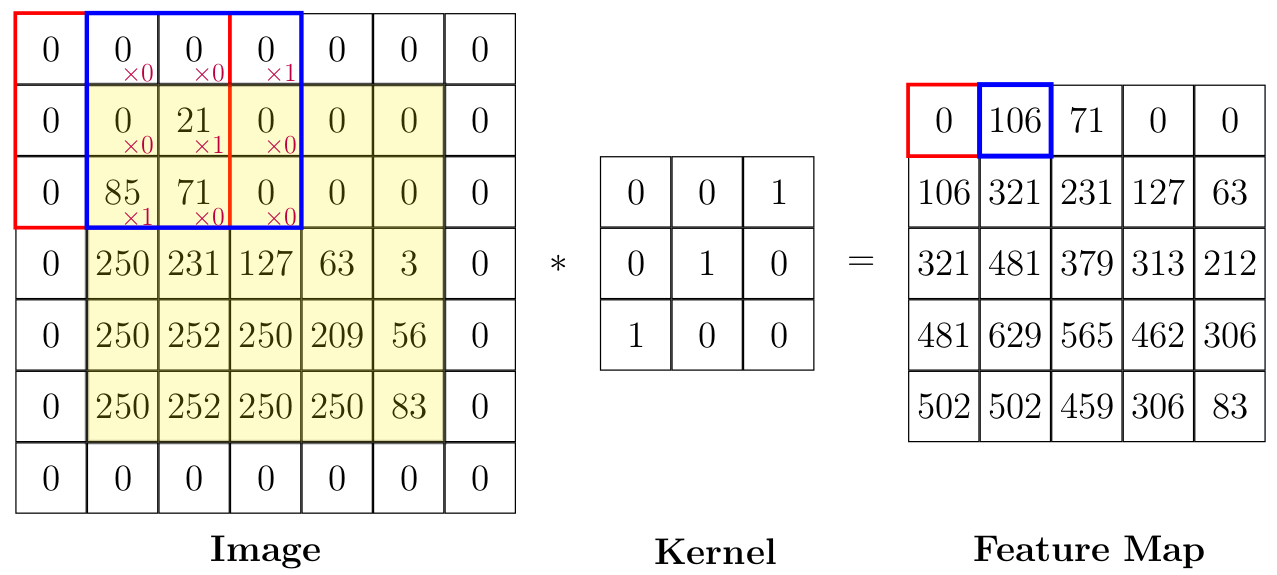
\includegraphics[width=0.9\textwidth]{convnet.png}
	\end{figure}
\end{frame}
				
				
\section{Related Works}
\begin{frame}[plain]
	\centering
	\huge
	\textsc{\color{blue}Related Works}
\end{frame}

\begin{frame}{Metric Learning}
	\begin{figure}
		\only<1>{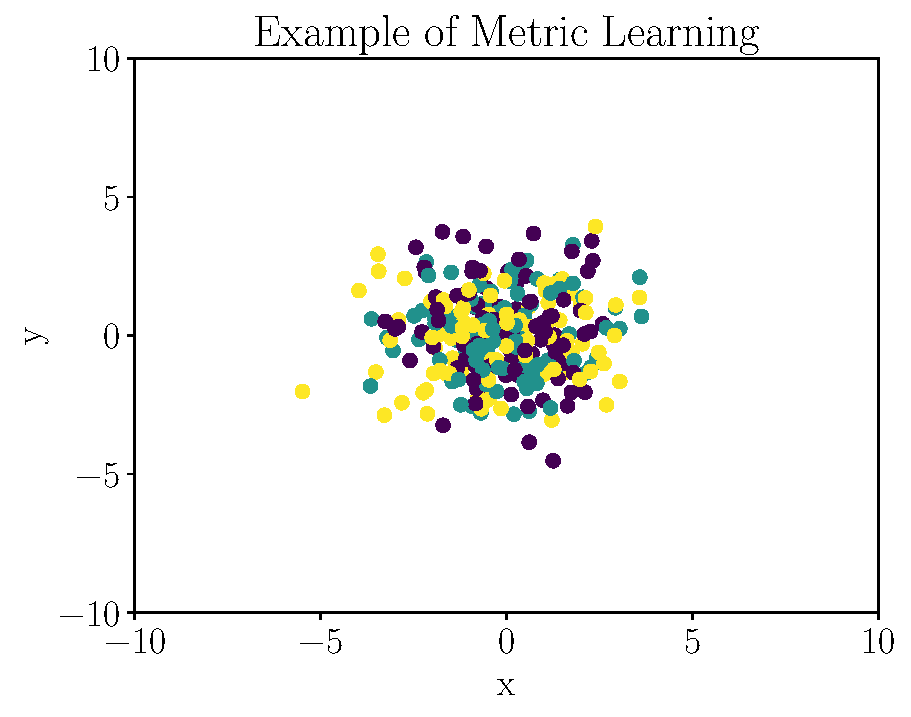
\includegraphics[width=0.8\textwidth]{plot1.pdf}}
		\only<2>{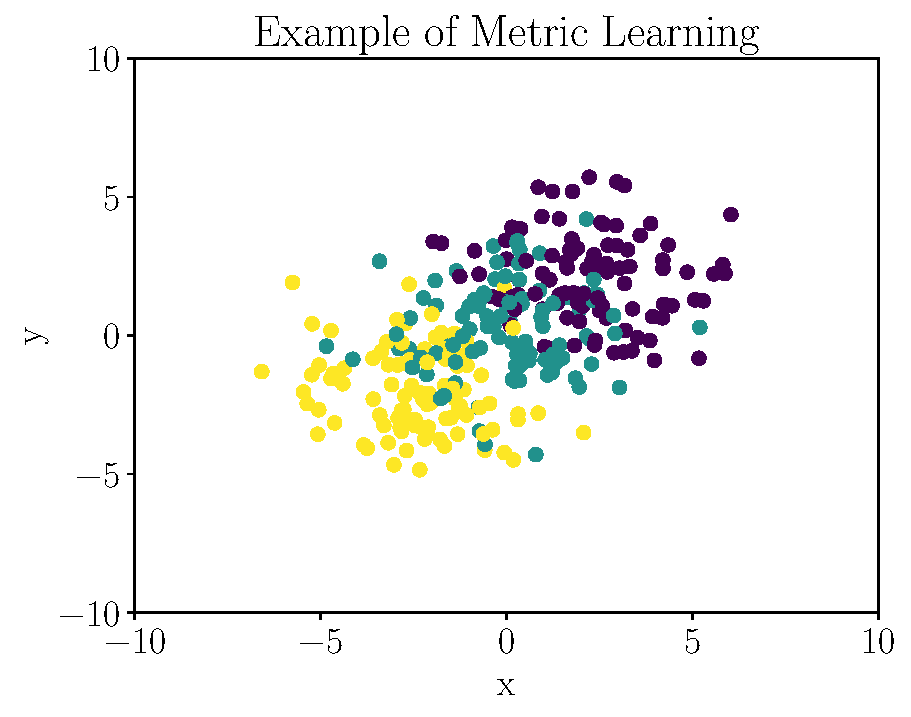
\includegraphics[width=0.8\textwidth]{plot2.pdf}}
		\only<3>{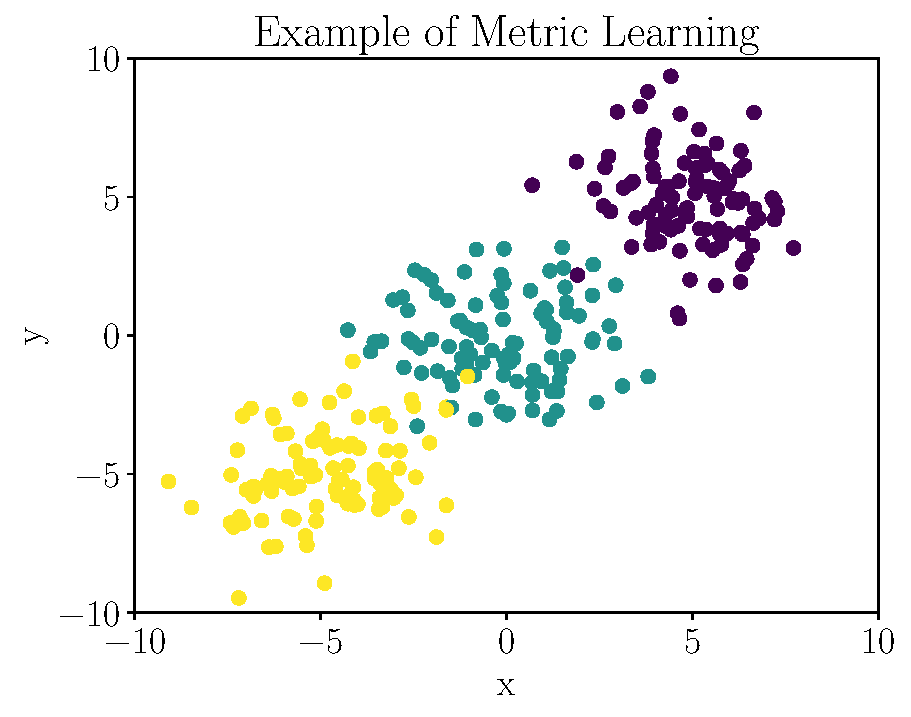
\includegraphics[width=0.8\textwidth]{plot3.pdf}}
	\end{figure}
\end{frame}

\begin{frame}{Contrastive Loss}
	\begin{itemize}
		\item \cite{hadsell2006dimensionality} minimize the distance between a pair of examples with same class label and penalizes the the negative pair distance
		\item Illustration of contrastive learning:
		\begin{figure}
			\centering
			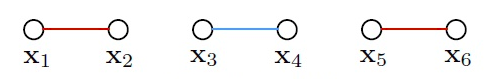
\includegraphics[width = 0.8\textwidth]{contrastive_learning.png}
		\end{figure}
		\item Mathematically, 
		$$ J = \frac{1}{m} \sum_{(i,j)}^{m/2} y_{i,j} D_{i,j}^2  + (1-y_{i,j}) [\alpha - D_{i,j}]_{+}^2$$
	\end{itemize}
\end{frame}

\begin{frame}{Triplet Loss}
	\begin{itemize}
		\item \cite{facenet} minimize distance between similar inputs and maximize distances between dissimilar inputs
		\item How do we know whether a signal is similar? With labels!
		\item Anchor, an instance of class $a$; positive, an instance of class $a$; negative, an instance of class $b$
		      \begin{figure}
		      	\centering
		      	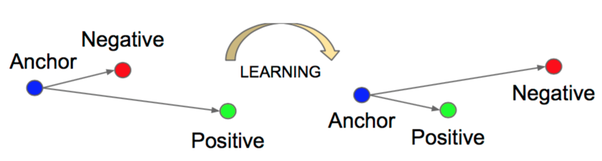
\includegraphics[width = 0.8\textwidth]{tripletloss.png}
		      \end{figure}
		      \item{
		            Mathematically, 
		            $$ J = \sum_{(a, p, n)}^N D_{a,p}^2 - D_{a,n}^2 +  \alpha $$
		      }
	\end{itemize}
\end{frame}

\begin{frame}[t]{Lifted Structure Embedding}
	\begin{itemize}
		\item \cite{structuredfeatureembedding} attempt to learn an embedding by looking at all possible pairs of related pairs in a minibatch
		\item Worked very well but more complicated than Triplet loss
	\end{itemize}
	\begin{equation*}
		\begin{gathered}
			\tilde{J}_{i,j} = log \bigg( \sum_{(i,k) \in \mathcal{N}} \exp\{ \alpha - D_{i,k} \} + \sum_{(j,l) \in \mathcal{N}} \exp\{\alpha - D_{j, l}\} \bigg) + D_{i, j}
			\\
			J = \frac{1}{2 |\mathcal{P}|} \sum_{(i,j) \in \mathcal{P}} \max \Big( 0, \tilde{J}_{i,j}\Big)^2
		\end{gathered}
	\end{equation*}
	
	\begin{figure}
		\centering
		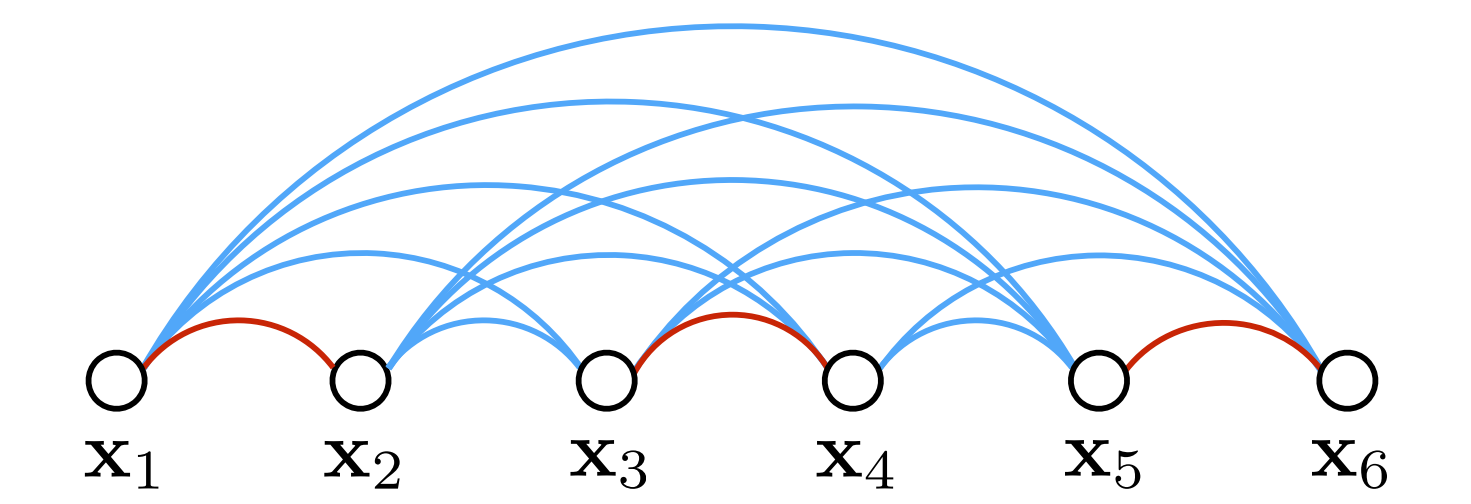
\includegraphics[width = 0.8\textwidth]{lifted_structured_embedding.png}
	\end{figure}
\end{frame}

				
\section{Data}
\begin{frame}[plain]
	\centering
	\huge
	\textsc{\color{blue}Data}
\end{frame}
\begin{frame}{Electroencephalography (EEG)}
	\begin{columns}
		\begin{column}{0.6\textwidth}
			\begin{itemize}
				\item Method of measuring electrical activity in the brain
				\item Helps diagnose variety of diseases
				\item Has standard, 10-20 placement
				\item Montages, differences in voltages, are used in medicine
				\item Frequency, phase, amplitude, location all are import sources of information an an EEG 			
				\item Our data is derived from TUH EEG Corpus	
			\end{itemize}	
		\end{column}
																																				
		\begin{column}{0.5\textwidth}									
			\begin{figure}
				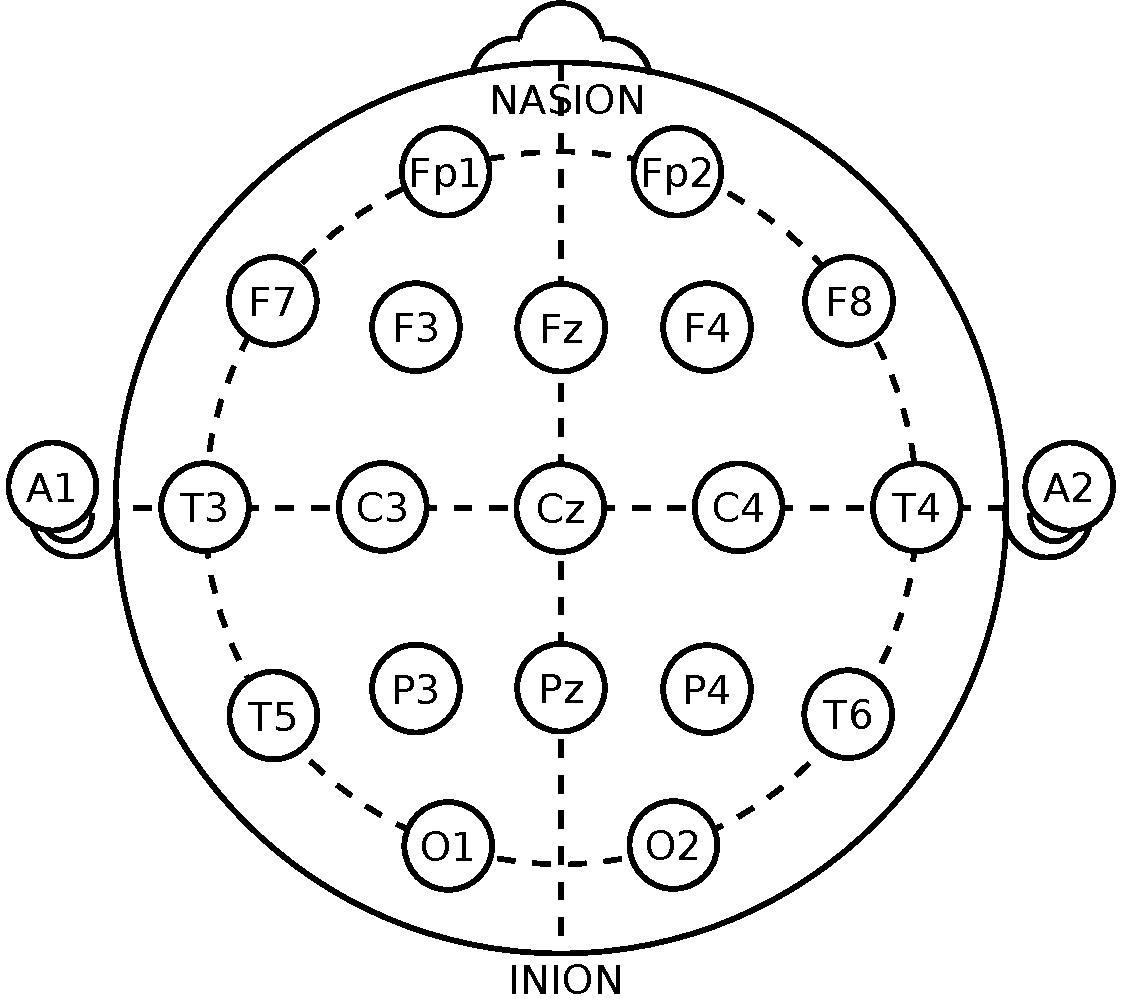
\includegraphics[width = 0.8\columnwidth]{tentwenty.pdf}
			\end{figure}
		\end{column}
	\end{columns}
\end{frame}
				
\begin{frame}{PSD of Sample from TUH EEG Corpus}
	\begin{figure}
		\centering
		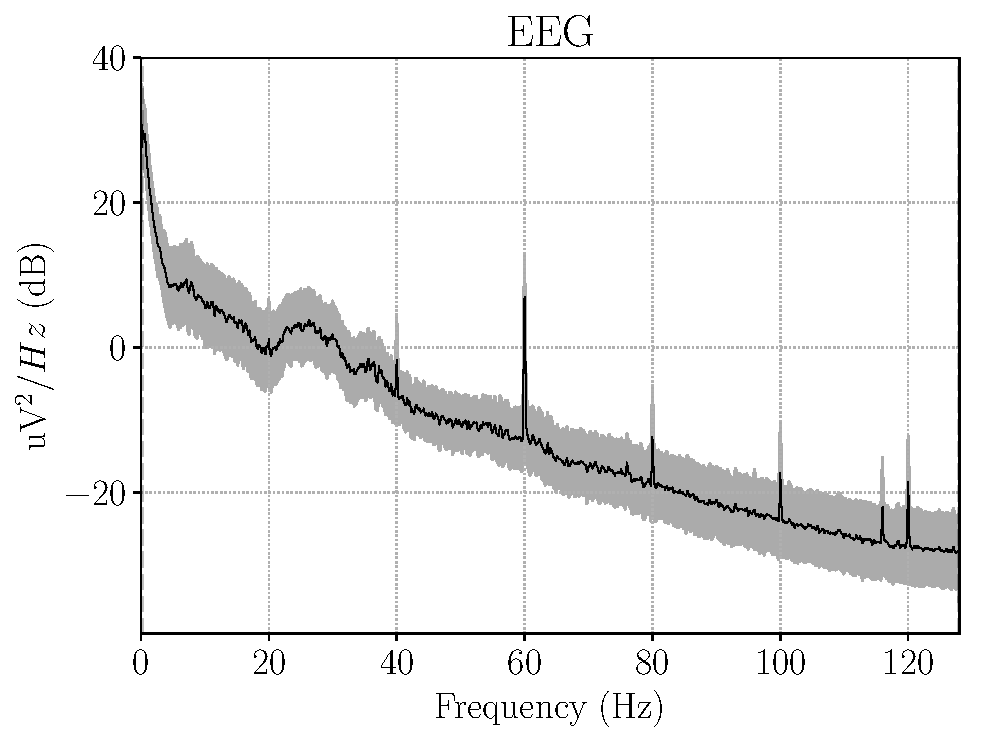
\includegraphics[width = 0.8\textwidth]{psd.pdf}
	\end{figure}
\end{frame}
				
\begin{frame}{Data Rectification}
	\begin{itemize}
		\item Notch filtered at 60 Hz
		\item Bandpass filtered with 1 - 70 Hz passband
		\item STFT with window of 140 samples \& stride of 2 samples
		\item Resulted in a $71 \times 125$ matrix for each second of the EEG 
		\item Omitted locations due to classification inconsistencies
		\item Split into mutually exclusive training and validation set of 85\% and 15\% respectively 
		      %%\item Globally normalized s	ignal power
	\end{itemize}
	\vspace*{-2em}
	\begin{table}
		\centering
		\huge
		\resizebox{\columnwidth}{!}{%
			\begin{tabular}{lm{14cm}l}
				\cmidrule{1-2}
				Code & Description                                  &                                                       \\ \cmidrule{1-2}
				BCKG & Background noise                             & \multirow{3}{*}{$\left. \vphantom{\begin{tabular}{c}3 \\3\\3\end{tabular}}\right\}$Noise-Like}\\
				ARTF & Artifacts                                    &                                                       \\
				EYBL & Eyeball movement                             &                                                       \\
				SPSW & Spikes \& sharp waves                        & \multirow{3}{*}{$\left. \vphantom{\begin{tabular}{c}3 \\3\\3\end{tabular}}\right\}$Seizure-Like}\\
				PLED & Periodic lateralized epileptiform discharges &                                                       \\
				GPED & Generalized periodic epileptiform discharges &                                                       \\\cmidrule{1-2}
			\end{tabular}
		}
		\label{tab:classes}
	\end{table}
\end{frame}
				
\begin{frame}{Resulting Matrix}
	\begin{figure}
		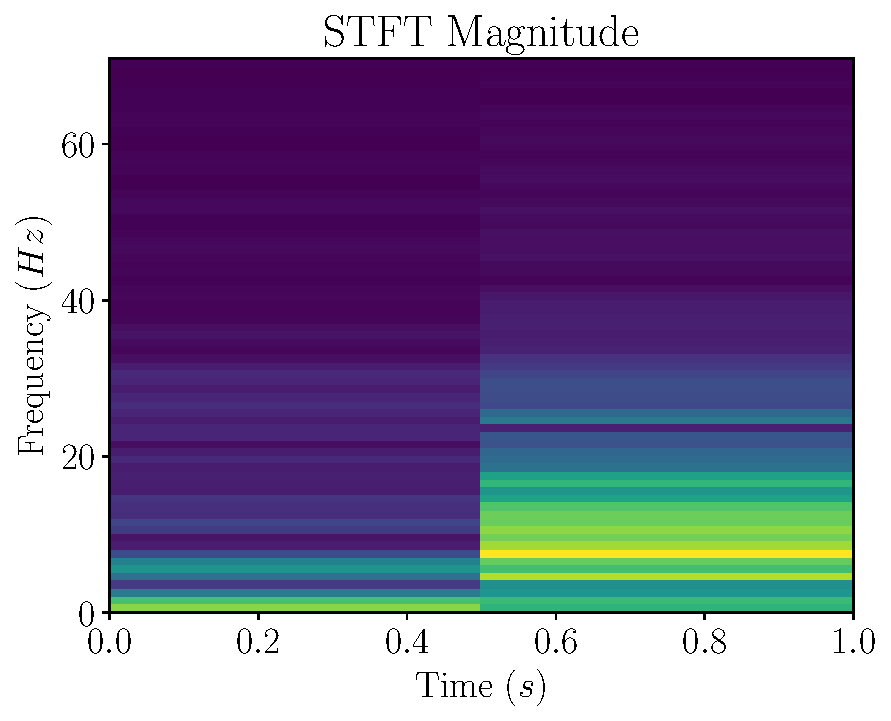
\includegraphics[width = 0.8\textwidth]{plot21.pdf}
	\end{figure}
\end{frame}   
				
				
\section{Experiments}
\begin{frame}[plain]
	\centering
	\huge
	\textsc{\color{blue}Experiments and Results}
\end{frame}
				
\begin{frame}{Experimental Design Choices}
	\begin{itemize}
		\item Is deep learning appropriate for this problem?
		      \begin{itemize}
		      	\item Dealing with unstructured data
		      \end{itemize}
		\item Which technique can we use to train the network?
		      \begin{itemize}
		      	\item Triplet Loss because it's simple yet effective
		      	\item Relatively easy to mine for triplets
		      \end{itemize}
		\item What type of network do we choose?
		      \begin{itemize}
		      	\item Convolutional Neural Network
		      	\item CNNs tend to do well on images
		      \end{itemize}
		\item How do we test the results? 
		      \begin{itemize}
		      	\item Classification using k-Nearest Neighbors
		      	\item Visualize latent space using t-SNE in 2D
		      	\item Compare to baseline classifier
		      \end{itemize}
	\end{itemize}
\end{frame}
				
\begin{frame}{Intial Experiment}
	\begin{columns}
		\begin{column}{0.6\textwidth}
			\begin{itemize}
				\item Designed simple CNN and implemented in TensorFlow
				\item Initially converged to zero due to small values and stalling triplet selection
				\item Amplified inputs to prevent both mistakes and speed up learning
				      				      				      				      				      					      					      					      					      				      				      				      				
			\end{itemize}	
		\end{column}
																																				
		\begin{column}{0.5\textwidth}									
			\footnotesize								
			\begin{table}[!ht]
				\centering
				\begin{tabular}{rll}\toprule
					Layer  & Input                       & Kernel         \\ \midrule
					conv1  & $ 71 \times 125 \times 1 $  & $ 4 \times 4 $ \\
					pool1  & $ 71 \times 125 \times 32 $ & $ 3 \times 3 $ \\
					conv2  & $ 35 \times 62 \times 32  $ & $ 5 \times 5 $ \\
					pool2  & $ 35 \times 62 \times 64 $  & $ 2 \times 2 $ \\
					fc1    & $17 \times 30 \times 64$    & N/A            \\
					fc2    & $ 256 $                     & N/A            \\
					output & $ 128 $                     & N/A            \\ \bottomrule
				\end{tabular}
				\label{tab:network}
			\end{table}
		\end{column}
	\end{columns}
\end{frame}
				
\begin{frame}{Intial Experiment}
	\begin{columns}
		\begin{column}{0.6\textwidth}
			\textbf{Hyperparameter Optimization}
			\begin{itemize}
				\item Optimized hyperparameters based on manual gridsearch
				      \begin{itemize}
				      	\item $\eta = 10^{-3}, \lambda_{L_2} = 10^{-4}$
				      	\item $d=128, \alpha = 1.0$
				      \end{itemize}
				\item Trained for $60$k steps 				      				
			\end{itemize}	
			\textbf{Measuring Performance}
			\begin{itemize}
				\item Used k-NN with $k=5$ to classify signals and calculate accuracies
				\item Resulted in 80\% accuracy 
			\end{itemize}
			\textbf{Error Organizing Data}
			\begin{itemize}
				\item Different classes were split, but sessions were not
			\end{itemize}
		\end{column}
																																				
		\begin{column}{0.5\textwidth}									
			\footnotesize								
			\begin{table}[!ht]
				\centering
				\begin{tabular}{rll}\toprule
					Layer  & Input                       & Kernel         \\ \midrule
					conv1  & $ 71 \times 125 \times 1 $  & $ 4 \times 4 $ \\
					pool1  & $ 71 \times 125 \times 32 $ & $ 3 \times 3 $ \\
					conv2  & $ 35 \times 62 \times 32  $ & $ 5 \times 5 $ \\
					pool2  & $ 35 \times 62 \times 64 $  & $ 2 \times 2 $ \\
					fc1    & $17 \times 30 \times 64$    & N/A            \\
					fc2    & $ 256 $                     & N/A            \\
					output & $ 128 $                     & N/A            \\ \bottomrule
				\end{tabular}	
			\end{table}
		\end{column}
	\end{columns}
\end{frame}
				
				
\begin{frame}{Deeper Convolutional Network}
	\begin{columns}
		\begin{column}{0.5\textwidth}
			\begin{itemize}						
				\item Designed network with 14 layers
				\item Convolutions followed by maxpool layers and fully connected layers
				\item Results in a 64 dimension vector representing the signal in embedding space
				\item Utilized same triplet loss to optimize network
			\end{itemize}
		\end{column}
																																				
		\begin{column}{0.6\textwidth}
																																																				
			\footnotesize																					
			\begin{table}[!ht]
				\centering
				\begin{tabular}{rllc}\toprule
					Layer    & Input                     & Kernel       \\ \midrule
					conv1    & $71 \times 125 \times 1$  & $5 \times 5$ \\
					maxpool1 & $71 \times 125 \times 32$ & $5 \times 5$ \\
					conv2    & $34 \times 61 \times 32$  & $3 \times 3$ \\
					maxpool2 & $34 \times 61 \times 64$  & $3 \times 3$ \\
					conv3    & $16 \times 30 \times 64$  & $2 \times 2$ \\
					maxpool3 & $16 \times 30 \times 128$ & $2 \times 2$ \\
					conv4    & $8 \times 15 \times 128$  & $1 \times 1$ \\
					maxpool4 & $8 \times 15 \times 256$  & $2 \times 2$ \\
					conv5    & $4 \times 7 \times 256$   & $4 \times 4$ \\
					maxpool5 & $4 \times 7 \times 1024$  & $4 \times 4$ \\
					flatten  & $1 \times 2 \times 1024$  & N/A          \\
					fc1      & 2048                      & N/A          \\
					fc2      & 1024                      & N/A          \\
					fc3      & 512                       & N/A          \\
					fc4      & 256                       & N/A          \\
					output   & 64                        &              \\\bottomrule
				\end{tabular}
			\end{table}
		\end{column}
	\end{columns}
\end{frame}
				
\begin{frame}{Deeper Convolutional Network}
	\begin{columns}
		\begin{column}{0.5\textwidth}
			\textbf{Hyperparameter Selection}
			\begin{itemize}
				\item Optimized hyperparameters based on manual gridsearch
				      \begin{itemize}
				      	\item $\eta = 10^{-5}, \lambda_{L_2} = 10^{-3}$
				      	\item $d=64, \alpha = 0.5$
				      \end{itemize}
				\item Trained for $105$k steps 	
			\end{itemize}	
			\textbf{Measuring Performance}
			\begin{itemize}
				\item Same procedure with k=31
				\item Resulted in 60.4\% 6-class and 90.4\% 2-class accuracy
				\item Constructed t-SNE reduced plots 
			\end{itemize}      				
												
		\end{column}
																																				
		\begin{column}{0.6\textwidth}						
			\footnotesize								
			\begin{table}[!ht]
				\centering
				\begin{tabular}{rllc}\toprule
					Layer    & Input                     & Kernel       \\ \midrule
					conv1    & $71 \times 125 \times 1$  & $5 \times 5$ \\
					maxpool1 & $71 \times 125 \times 32$ & $5 \times 5$ \\
					conv2    & $34 \times 61 \times 32$  & $3 \times 3$ \\
					maxpool2 & $34 \times 61 \times 64$  & $3 \times 3$ \\
					conv3    & $16 \times 30 \times 64$  & $2 \times 2$ \\
					maxpool3 & $16 \times 30 \times 128$ & $2 \times 2$ \\
					conv4    & $8 \times 15 \times 128$  & $1 \times 1$ \\
					maxpool4 & $8 \times 15 \times 256$  & $2 \times 2$ \\
					conv5    & $4 \times 7 \times 256$   & $4 \times 4$ \\
					maxpool5 & $4 \times 7 \times 1024$  & $4 \times 4$ \\
					flatten  & $1 \times 2 \times 1024$  & N/A          \\
					fc1      & 2048                      & N/A          \\
					fc2      & 1024                      & N/A          \\
					fc3      & 512                       & N/A          \\
					fc4      & 256                       & N/A          \\
					output   & 64                        &              \\\bottomrule
				\end{tabular}
			\end{table}
		\end{column}
	\end{columns}
\end{frame}
				
% \begin{frame}{Evaluating Results}
% 	\begin{itemize}
% 		\item Measured discriminative power of the latent space with a k-NN classifier
% 		\item Found embeddings of randomly sampled training and testing data embeddings with network
% 		\item Populated k-NN space with training embeddings and classified testing embeddings
% 		\item Calculated confusion matrices, accuracies and utilized t-SNE to visualize dimensionality-reduced embeddings
% 		\item Resulted in a $60.4\%$ overall accuracy
% 	\end{itemize}
% \end{frame}
				
\begin{frame}{t-SNE Plot at 5k Iterations}
	\centering
	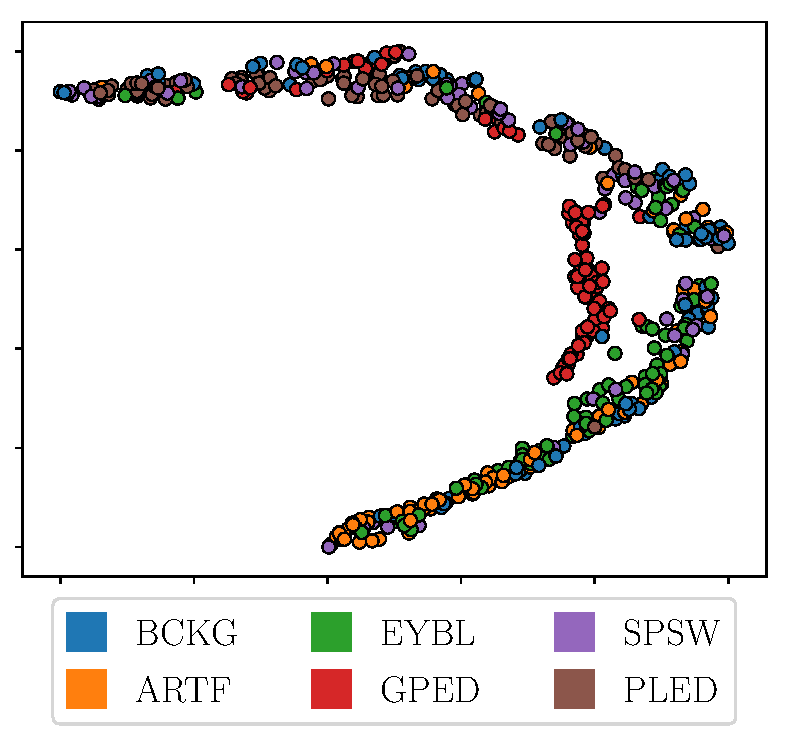
\includegraphics[width=0.7\textwidth,keepaspectratio]{tsne_plot_start.pdf}
\end{frame}

\begin{frame}{t-SNE Plot at 105k Iterations}
	\centering
	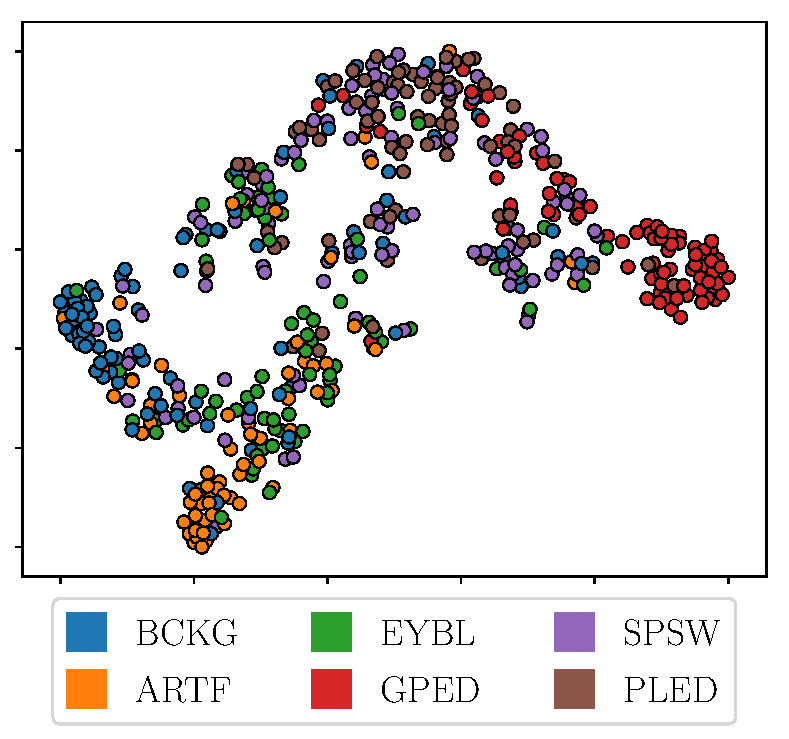
\includegraphics[width=0.7\textwidth,keepaspectratio]{tsne_plot.pdf}
\end{frame}
				
\begin{frame}{Confusion Matrix for Six-Class Classification}
	\centering
	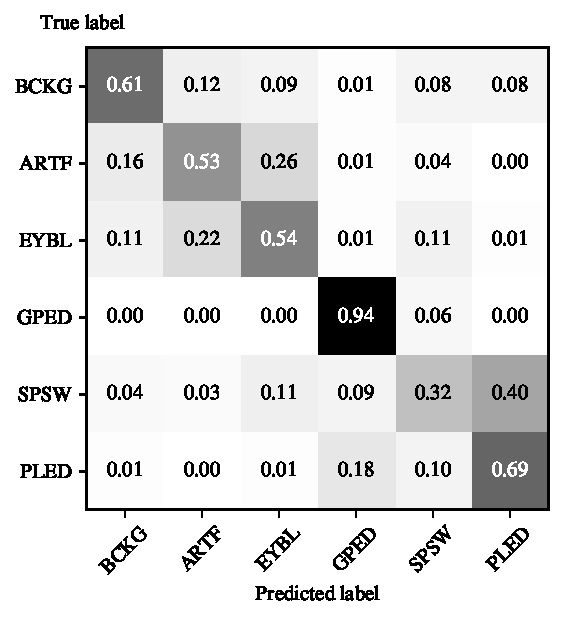
\includegraphics[height=0.6\textwidth,keepaspectratio]{conf_mat_exp.pdf}
\end{frame}
				
\begin{frame}{t-SNE Plot with Binary Decision Boundary}
	\centering
	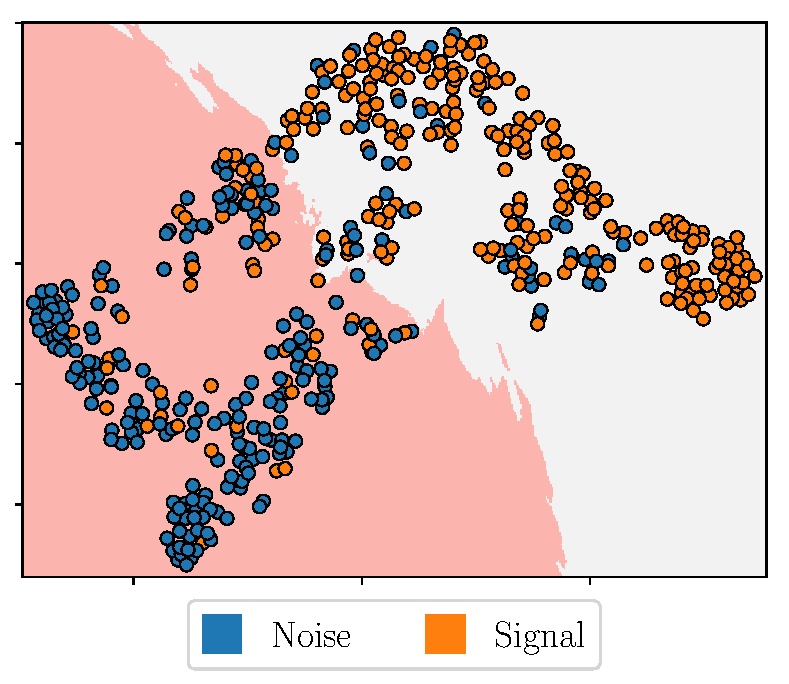
\includegraphics[height=0.6\textwidth,keepaspectratio]{tsne_plot_binary.pdf}
\end{frame}
				
\begin{frame}{Confusion Matrix for Binary Classification}
	\centering
	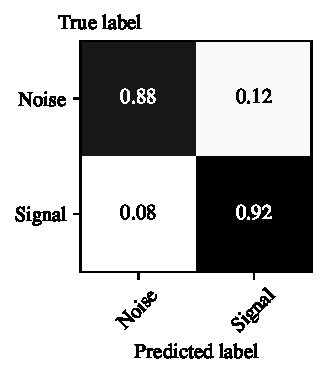
\includegraphics[height=0.6\textwidth,keepaspectratio]{conf_mat_exp_pooled.pdf}
\end{frame}

\begin{frame}{DCNN with Softmax Loss}
	\begin{columns}
		\begin{column}{0.5\textwidth}
			\begin{itemize}
				\item Created a DCNN classifier
				\item Utilized same network
				\item Applied cross-entropy loss
				\item Resulted in classification accuracy of $50.2\%$
				\item Surprising results
			\end{itemize}	
		\end{column}
																																				
		\begin{column}{0.5\textwidth}									
			\begin{figure}
				\hbox{\hspace{-0.5em} 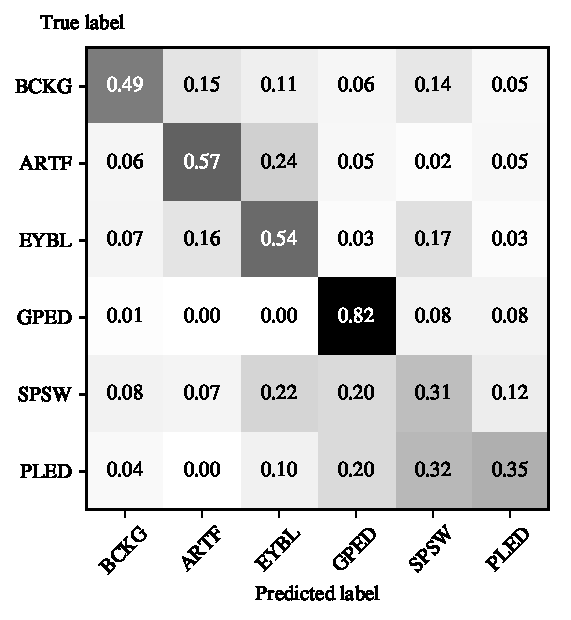
\includegraphics[height=1.2\columnwidth,keepaspectratio]{conf_mat_baseline.pdf}}
			\end{figure}
		\end{column}
	\end{columns}
		
\end{frame}
				

				
\begin{frame}{Error Analysis}
	\begin{itemize}
		\item Analyze where most error occurs
		\item Split dataset into three sectors: 
		      \begin{itemize}
		      	\item Type A: Sessions without seizure-like signals
		      	\item Type B: Sessions with seizure-like signals
		      	\item Type C: Sessions with seizure-like signals considering \\ only seizure-like signals
		      \end{itemize}
		\item Try to identify reasons why these errors occur
		\item Splitting them helps identify how the changes in sessions changes results
	\end{itemize}
\end{frame}		

\begin{frame}{Error Analysis: Type A (64.6\% and 93.0\%)}
	\begin{columns}
		\begin{column}{0.6\textwidth}
			\centering
			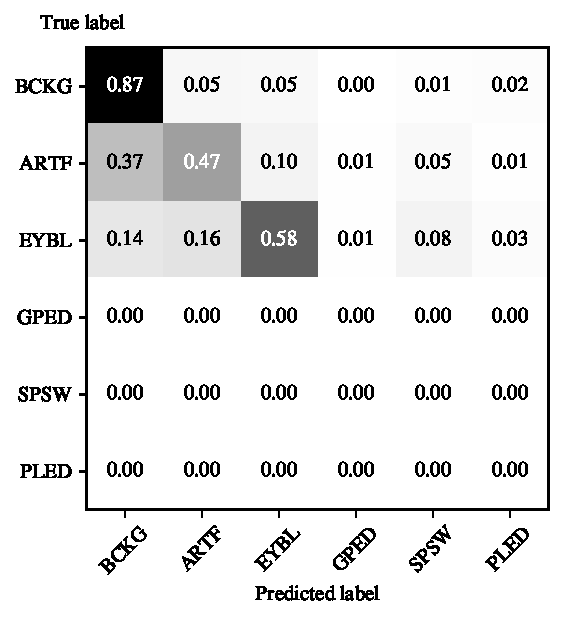
\includegraphics[width=\textwidth]{conf_mat_exp_without_seizure.pdf}
		\end{column}
																																				
		\begin{column}{0.4\textwidth}
			\centering
			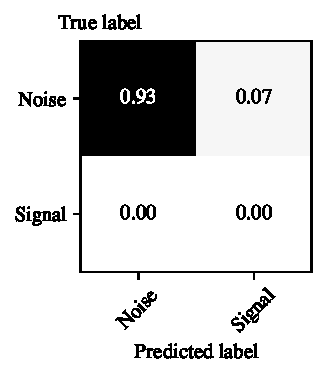
\includegraphics[width=\textwidth]{conf_mat_exp_without_seizure_pooled.pdf}
		\end{column}
	\end{columns}
\end{frame}	

\begin{frame}{Error Analysis: Type B (56.0\% and 85.0\%)}
	\begin{columns}
		\begin{column}{0.6\textwidth}
			\centering
			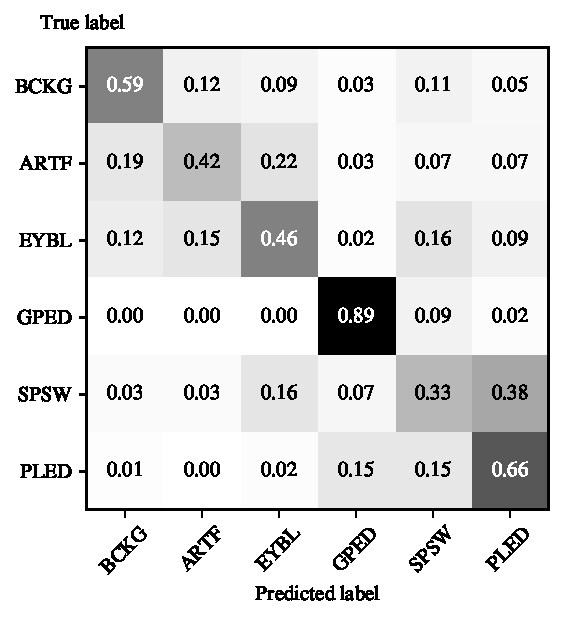
\includegraphics[width=\textwidth]{conf_mat_exp_with_seizure.pdf}
		\end{column}
																																				
		\begin{column}{0.4\textwidth}
			\centering
			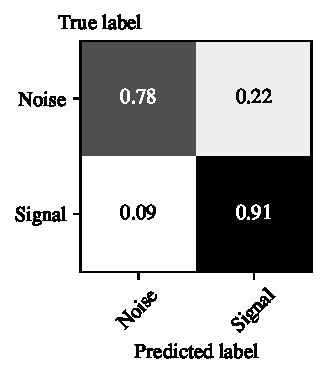
\includegraphics[width=\textwidth]{conf_mat_exp_with_seizure_pooled.pdf}
		\end{column}
	\end{columns}
\end{frame}	

\begin{frame}{Error Analysis: Type C (63.0\% and 91.8\%)}
	\begin{columns}
		\begin{column}{0.6\textwidth}
			\centering
			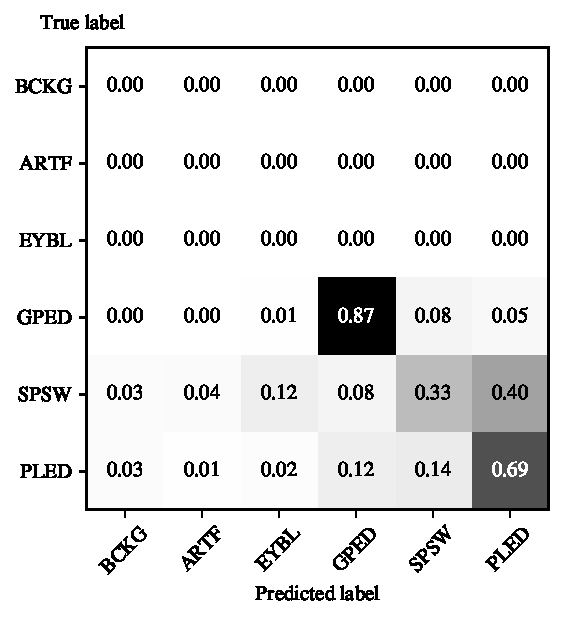
\includegraphics[width=\textwidth]{conf_mat_exp_with_only_seizure.pdf}
		\end{column}
																																				
		\begin{column}{0.4\textwidth}
			\centering
			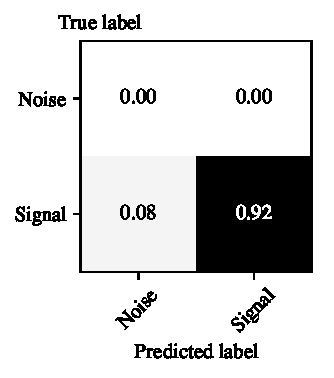
\includegraphics[width=\textwidth]{conf_mat_exp_with_only_seizure_pooled.pdf}
		\end{column}
	\end{columns}
\end{frame}	


\begin{frame}{Possible Sources of Error}
	\begin{itemize}
		\item Misclassified signals
		\item Very similar signals
		\item Loss of information due to:
		      \begin{itemize}
		      	\item Notch filter
		      	\item Bandpass filter
		      	\item Magnitude of STFT
		      	\item Location on scalp
		      \end{itemize}
		\item \textbf{However,} accuracy is still high for a signal with low SNR	
	\end{itemize}
\end{frame}	
				
				
				
\section{Conclusion}
\begin{frame}{Conclusions and Future Work}
	\begin{itemize}
		\item Demonstrated an end-to-end system to learn latent spaces for EEG signals
		\item 60.4\% six-class \& 90.4\% binary classification accuracies
		\item Does better than generic DCNN classifier and provides more information on similarity
		\item Experiment swapping triplet loss with loss functions from Structured Feature Embeddings written \cite{structuredfeatureembedding}
		\item Do an in-depth analysis between features produced by baseline and those produced by experimental network
		\item Attempt to incorporate physicians' notes in order to enrich embeddings produced using adaptive density discrimination
		\item Extend this method to other types of medical signals and enrich understanding of different pathologies
	\end{itemize}
\end{frame}
				
\section{Acknowledgements}
\begin{frame}{Thank you to...}
	\begin{itemize}
		\item Professor Sam Keene
		\item Chris Curro
		\item ECE Faculty
		\item My friends
		\item My parents
	\end{itemize}
\end{frame}

\begin{frame}[plain]
	\centering
	\huge
	\textsc{\color{blue}Questions?}
\end{frame}

\end{document}